\section{Control System}
The goal of having a prostheses that makes the life of the user easier. Since "the solution with the biggest potential to improve the users life is an electric prostheses a question comes to mind. How should such a prothesis be controlled by the user, in order to reach the goal. 
Norman S. Nise define a control system in his book Nises' Control System Engineering and provides 4 resons to use a control system:\\
\begin{displayquote}
 \textit{"A control system consist of subsystems and processes assembled for the purpose of obtaining a desired output with desired performance given a specific input\\[...]\\ We build control systems for four primary reasons. 
\begin{enumerate}
    \item Power amplification
    \item Remote control
    \item Convenience of input form
    \item Compensation of disturbances "
\end{enumerate}}\hspace{0.65\textwidth} -Norman S. Nise \cite{Nise}
\end{displayquote} \label{Quote1}
\noindent The need of a control system is clear in this project. Remote control allows compensation for the missing limb. Sense the input can be selected by convince the project can can choose any interface. All of which is useful for the end user. There is many different kinds of control systems, an elaboration of which is used in this project can be seen in Chapter \ref{ch:Design} describing the design of the system. 
\subsection*{Interfaces}
The user of a control system allows for any input. It is therefore relevant to look into different interfaces that can be used to control the manipulator:

\subsubsection*{Surface electromyography}\label{sEMG}
sEMG or surface electromyography, is a way of interpreting the signals given when muscular activities occur. sEMG signals can be read by applying electrodes to the muscle, when the muscle contracts a wave is sent through the electrodes and then viewed in the application used on the device reading it.\\
In figure \ref{fig:sEMG}, we can interpret the sinoid wave and determine the characteristics of it:

\begin{figure}[H]
    \centering
    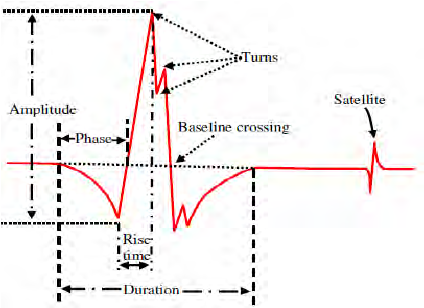
\includegraphics[width=12cm,height=7cm]{Figures/Contextual_figures/Characteristics-of-EMG-signal.png}
    \caption{sEMG \cite{sEMG}}
    \label{fig:sEMG}
\end{figure}

\begin{itemize}
  \item \textbf{Amplitude} determines how intense your muscle contracts.
    \item \textbf{Phase}  describes the delay or overlay in the waves. If the waves are in phase they are 0 or 360 degrees apart, which means they overlap. Waves with shift phase can be visually seen and determined how far apart the waves are.
    \item \textbf{Rise Time} is a measurement to determine a rise in the wave, from 10 percent to 90 percent.
    \item \textbf{Duration} can be described as a single oscillation of the sin-wave.
\end{itemize}

Some of the benefits to controlling a system with a sEMG is the ease of use for the user, it is a non invasive system and depending on the programming the system can be fairly intuitive to use, while still be easy to equip. 
Some downside are there though.one being the noise of the data-stream. this control method requires the need of filters to interpret the inputs into usable data. Another is the need for a skintight seal on the muscle which can result in several difficulties see section \ref{Difficoulties}.

\subsubsection{Accelerometers}
Accelerometers measure the acceleration of gravity, with this information the orientation of the accelerometer can be calculated.\\
Systems such as the Inertial Measurement Unit(IMU) and Inertial Navigation System (INS) uses a combination of sensors such as accelerometers and gyroscopes to detect changes in roll, pitch and yaw and in linear acceleration\cite{IMUWorki40:online}.\\ These are often used in planes and ships and can be used as inputs in a controller\\ 
This method have similar benefits to the sEMG, its small and easy for the user, but the signal needs processing to interpret.
\\ 
\subsubsection*{Eye-tracking}
Eye tracking is a devise used to interpret where the gaze of the user is directed. 

\begin{figure}[H]
    \centering
    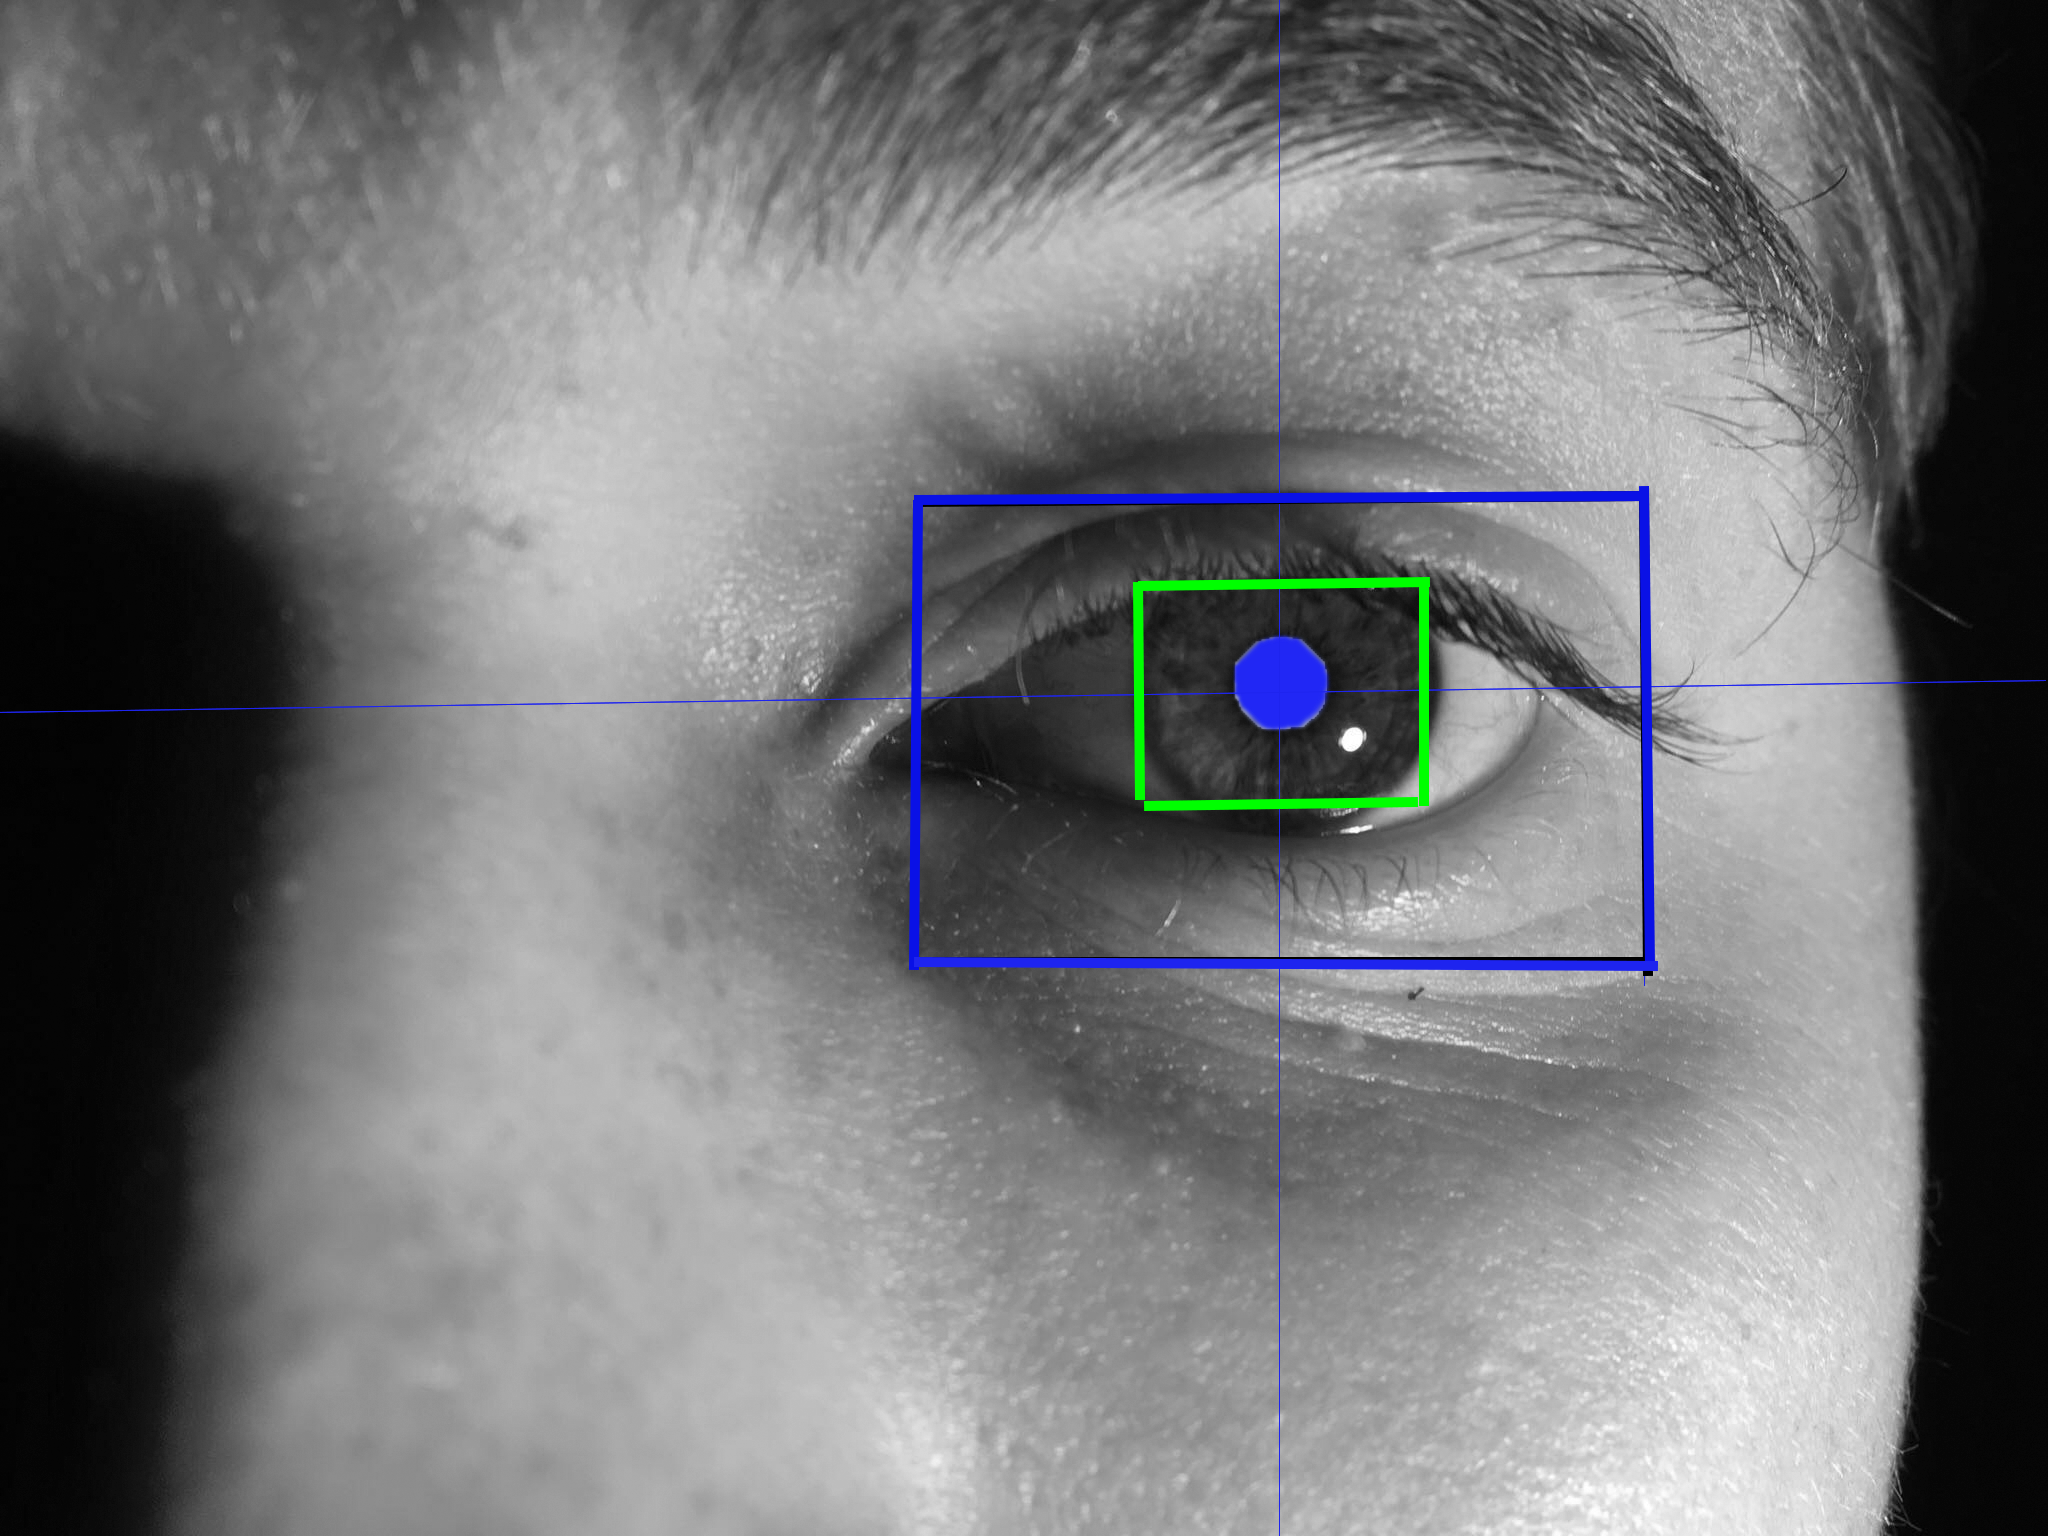
\includegraphics[width=10cm,height=7cm]{Figures/Contextual_figures/eye-tracking.png}
    \caption{Eye-tracking}
    \label{fig:Eye}
\end{figure}

As seen in figure\ref{fig:Eye}, the devise will indulge the users pupil with a dim infrared light. When the pupil is lighted a infrared camera will catch the movement of the reflection and send the data to the devise which will use it to measure where the user is looking.\\
These features could be used to steer the arm towards desirable locations relying solely on eye-tracker \cite{EyeTrack}. There are some clear disadvantages to this interface. The device has detect the eye movement meaning that the ideal position is in front of the users face. There is also a chance of false positives where the user does not want to move the arm bur a sudden movement makes the user look in another direction causing the arm to move. 

\subsubsection*{Joystick}
A joystick can be used to control many things, such as wheelchairs, computers and many other devices. A joystick works through the use of potentiometers. A potentiometer is a variable resistor, when the joystick is moved in one direction, the resistances will change and the voltage drop over potentiometer changes. The voltage drop can use be to translate in to a control signal for the device it is used on. Some joysticks like the Jouse3 are made in combination with a sip and puff system\cite{Jouse}. A joystick i often used for a person how are in a wheelchair or have minimal to no motor coordination.\\ 
\begin{figure}[H]
    \centering
    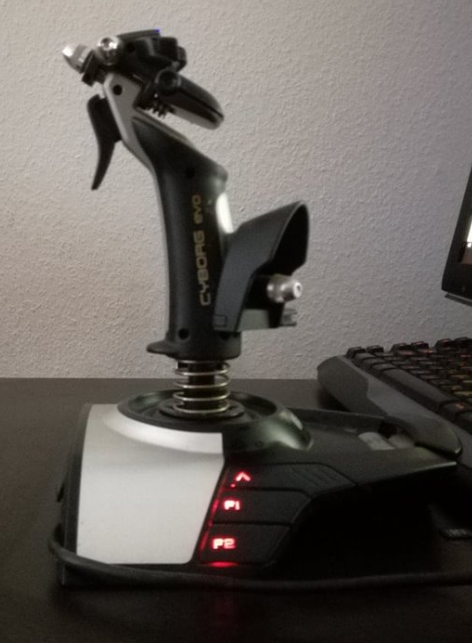
\includegraphics[width=5cm,height=7cm]{Figures/Contextual_figures/Joystickl.jpg}
    \caption{Joystick}
    \label{fig:picjoystick}
\end{figure}
The joystick mainly has two disadvantages. First of all it requires an arm to move. It is more convenient for the user to use the functional arm to do the movement rather than using the joystick thus making the interface redundant. Secondly prolonged use of a joystick can also lead to repetitive strain injuries. 
\subsubsection*{Sip-and-puff}
The sip and puff drive system use one or more pressure differential sensors.The User sip or blows through one straw an onto pressure differential sensors. Depending on sip and puff system and the way they are configured, some systems is only made for puff and sip where others can differentiate a slow sip or puffs from a hard sip or puffs. This all depends on the use of this system, it can be use on its own or in combination with others control systems\cite{Snp}. Most users for this system is wheelchair users like paraplegics or people with multiple scleroses.\\
\begin{figure}[H]
    \centering
    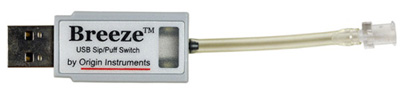
\includegraphics[width=9cm,height=3cm]{Figures/Contextual_figures/breeze_400.jpg}
    \caption{This photo was provided in courtesy of Origin Instruments \ref{st:Origin}\\ 
    Sip/Puff Breeze 400\cite{Snp}}
    \label{fig:Sip/Puff}
\end{figure}
The disadvantages of this system is the placement of the interface. The user cannot talk while operation the prostheses which is an annoyance to the user. 
\subsubsection*{I-tongue control system}
Thanks to the ever shrinking sizes of electronics, it is now possible to have a control system within the mouth in form of a retainer. The I-tongue control system from TKS\cite{TKS}, consists of two control areas one is a keyboard with 10 buttons, used as the "old mobile phone" where one button containing three or more letters and characters, the other control area on the I-tongue is a mouse pad and furthermore the user can select different control modes. A piercing is placed through the tongue of the user. When the user moves the piercing over the sensor, the signal for the sensor is transmitted through a wireless signal. The signal can be used to control almost any device. This is mostly used for tetraplegices or people with muscular failure like ALS\cite{TDSp}.\\
\begin{figure}[H]
    \centering
    \includegraphics[width=12cm,height=7cm]{}
    \caption{A view of how user could use the tongue to control a device\cite{TDSp}}
    \label{fig:TDS}
\end{figure}
the main disadvantage of this system is the operation needed in order to make this work. 
\subsubsection*{Safety precautions}

One way to ensure safety for the user, is to isolate the controller from the prostheses, so that if there is a short-circuit within the prostheses, the user do not have to fear for electrocution from the power source. This separation can be done in many ways, some is to use an isolating transformer\cite{isotrans} or through the use of a wireless signal like Bluetooth.  \\
Another way to ensure some safety for the user, is to keep the forces of prostheses minimised to a non-harmful level. Several experiments were done during WW2(The Second world war), where German doctors tested how much force could safely be applied without resulting in harm or even injury to people.\\  

\section{Conclusion} %Both prosthesis and control system 
Different viable options of prostheses' and control systems has been presented in the chapter above. By investigating these coherent options an understanding of existing solutions and viable system-controls can be reached.\\
Certain safety measures has been reviewed and a sub-conclusion has been taking into consideration. 